\section{EXPERIMENTS}
In this section, we conduct experiments on two widely used datasets to answer the following research questions:
\begin{itemize}
	\item RQ1: How does GRMM perform compared with different retrieval methods (typically traditional, local interaction-based, and BERT-based matching methods)?
	\item RQ2: How effective is the graph structure as well as the long-dependency in ad-hoc retrieval?
	\item RQ3: How sensitive (or robust) is GRMM with different hyper-parameter settings?
\end{itemize}

\subsection{Experiment Setup}
\subsubsection{Datasets.}
We evaluate our proposed model on two datasets: Robust04 and ClueWeb09-B.
\begin{itemize}
    \item Robust04\footnote{https://trec.nist.gov/data/cd45/index.html} is a standard ad-hoc retrieval dataset with 0.47M documents and 250 queries, using TREC disks 4 and 5 as document collections.
    \item ClueWeb09-B\footnote{https://lemurproject.org/clueweb09/} is the "Category B" subset of the full web collection ClueWeb09. It has 50M web pages and 200 queries, whose topics are accumulated from TREC Web Tracks 2009-2012.
\end{itemize}
Table \ref{tab:1} summarises the statistic of the two collections. For both datasets, there are two available versions of the query: a keyword title and a natural language description. In our experiments, we only use the title for each query.


\subsubsection{Baselines.}
To examine the performance of GRMM, we take three categories of retrieval models as baselines, including traditional (QL and BM25), local interaction-based (MP, DRMM, KNRM, and PACRR), and BERT-based (BERT-MaxP) matching methods, as follows: 

\begin{itemize}
    \item \textbf{QL} (Query likelihood model) \cite{zhai2004study} is one of the best performing language models that based on Dirichlet smoothing.
    \item \textbf{BM25} \cite{robertson1994some} is another effective and commonly used classical probabilistic retrieval model.
    \item \textbf{MP} (MatchPyramid) \cite{pang2016text} employs CNN to extract the matching features from interaction matrix, and dense neural layers are followed to produce final ranking scores.
    \item \textbf{DRMM} \cite{guo2016deep} performs a histogram pooling over the local query-document interaction signals. 
    \item \textbf{KNRM} \cite{xiong2017end} introduces a new kernel-pooling technique that extracts multi-level soft matching features.
    \item \textbf{PACRR} \cite{hui2017pacrr} uses well-designed convolutional layers and $k$-max-pooling layers over the interaction signals to model sequential word relations in the document.
    \item \textbf{Co-PACRR} \cite{hui2018co} is a context-aware variant of PACRR that takes the local and global context of matching signals into account.
    \item \textbf{BERT-MaxP} \cite{dai2019deeper} applies BERT to provide deeper text understanding for retrieval. The neural ranker predicts the relevance for each passage independently, and the document score is set as the best score among all passages.
\end{itemize}


\begin{table}[]
	\footnotesize
	\begin{tabular}{@{}ccccc@{}}
		\toprule
		\textbf{Dataset}     & \textbf{Genre} & \textbf{\# of qrys} & \textbf{\# of docs} & \textbf{avg.length} \\ \midrule
		\textbf{Robust04}    & news           & 250                 & 0.47M                & 460                         \\
		\textbf{ClueWeb09-B} & webpages       & 200                 & 50M                 & 1506                        \\ \bottomrule
	\end{tabular}
	\caption{Statistics of datasets.}
	\label{tab:1}
\end{table}


\subsubsection{Implementation Details.}
All document and query words were white-space tokenised, lowercased, and lemmatised using the WordNet\footnote{https://www.nltk.org/howto/wordnet.html}. We discarded stopwords as well as low-frequency words with less than ten occurrences in the corpus. Regarding the word embeddings, we trained 300-dimensional vectors with the Continuous Bag-of-Words (CBOW) model \cite{mikolov2013distributed} on Robust04 and ClueWeb-09-B collections. For a fair comparison, the other baseline models shared the same embeddings, except those who do not need. Implementation of baselines followed their original paper.

Both datasets were divided into five folds. We used them to conduct 5-fold cross-validation, where four of them are for tuning parameters, and one for testing \cite{macavaney2019cedr}. The process repeated five times with different random seeds each turn, and we took an average as the performance.

We implemented our method in PyTorch\footnote{Our code is at https://github.com/CRIPAC-DIG/GRMM}. The optimal hyper-parameters were determined via grid search on the validation set: the number of graph layers $t$ was searched in \{1, 2, 3, 4\}, the $k$ value of $k$-max-pooling was tuned in \{10, 20, 30, 40, 50, 60, 70\}, the sliding window size in \{3,5,7,9\}, the learning rate in \{0.0001, 0.0005, 0.001, 0.005, 0.01\}, and the batch size in \{8, 16, 32, 48, 64\}.
Unless otherwise specified, we set $t$ = 2 and $k$ = 40 to report the performance (see Section \ref{sec:neighbouraggre} and \ref{sec:featureelect} for different settings), and the model was trained with a window size of 5, a learning rate of 0.001 by Adam optimiser for 300 epochs, each with 32 batches times 16 triplets. All experiments were conducted on a Linux server equipped with 8 NVIDIA Titan X GPUs.

\subsubsection{Evaluation Methodology.}
Like many ad-hoc retrieval works, we adopted a re-ranking strategy that is more efficient and practical than ranking all query-document pairs. In particular, we re-ranked top 100 candidate documents for each query that were initially ranked by BM25. To evaluate the re-ranking result, we used the normalised discounted cumulative gain at rank 20 (nDCG@20) and the precision at rank 20 (P@20) as evaluation matrices. 


\subsection{Model Comparison (RQ1)}
Table \ref{tab:2} lists the overall performance of different models, from which we have the following observations:
\begin{itemize}
	\item GRMM significantly outperforms traditional and local interaction-based models, and it is comparable to BERT-MaxP, though without massive external pre-training. To be specific, GRMM advances the performance of nDCG@20 by 14.4\% on ClueWeb09-B much more than by 5.4\% on Robust04, compared to the best-performed baselines excluding BERT-MaxP. It is reasonably due to the diversity between the two datasets. ClueWeb09-B contains webpages that are usually long and casual, whereas Robust04 contains news that is correspondingly shorter and formal. It suggests that useful information may have distributed non-consecutively, and it is beneficial to capture them together, especially for long documents. GRMM can achieve long-distance relevance matching through the graph structure regardless of the document length. 
	
	\item On the contrary, BERT-MaxP performs relatively better on Robust04 than on ClueWeb09-B. We explain the observation with the following two points. First, since the input sequence length is restricted by a maximum of 512 tokens, BERT has to truncate those long documents from ClueWeb09-B into several passages. It, therefore, loses relations among different passages, i.e. the long-distance dependency. Second, documents from Robust04 are generally written in formal languages. BERT primarily depends on the pre-trained semantics, which could naturally gain benefit from that. 
	
	\item Regarding the local interaction-based models, their performances slightly fluctuate around the initial ranking result by BM25. However, exceptions are DRMM and KNRM on ClueWeb09-B, where the global histogram and kernel pooling strategy may cause the difference. It implies that the local interaction is insufficient in ad-hoc retrieval task. Document-level information also needs to be considered. 
	
	\item Traditional approaches like QL and BM25 remain a strong baseline though quite straightforward, which means the exact matching of terms is still of necessity as \citet{guo2016deep} proposed. These models also avoid the problem of over-fitting, since they do not require parameter optimisation. 
\end{itemize}                       

\label{sec:modelcompare}
\begin{table}[]
	\fontsize{9.3pt}{11pt}\selectfont
    \begin{tabular}{@{}cllll@{}}
    \toprule
    \multirow{2}{*}{Model} & \multicolumn{2}{c}{Robust04}                           & \multicolumn{2}{c}{ClueWeb09-B}                        \\ \cmidrule(l){2-5} 
                           & \multicolumn{1}{c}{nDCG@20} & \multicolumn{1}{c}{P@20} & \multicolumn{1}{c}{nDCG@20} & \multicolumn{1}{c}{P@20} \\ \midrule
    QL                     & 0.415$^-$                   & 0.369$^-$                & 0.224$^-$                   & 0.328$^-$                \\
    BM25                   & 0.418$^-$                   & 0.370$^-$                & 0.225$^-$                   & 0.326$^-$                \\ \midrule
    MP                     & 0.318$^-$                   & 0.278$^-$                & 0.227$^-$                   & 0.262$^-$                \\
    DRMM                   & 0.406$^-$                   & 0.350$^-$                & 0.271$^-$                   & 0.324$^-$                \\
    KNRM                   & 0.415$^-$                   & 0.359$^-$                & 0.270$^-$                   & 0.330$^-$                \\
    PACRR                  & 0.415$^-$                   & 0.371$^-$                & 0.245$^-$                   & 0.278$^-$                \\
    Co-PACRR               & 0.426$^-$                   & 0.378$^-$                & 0.252$^-$                   & 0.289$^-$                \\ \midrule
    BERT-MaxP              & \textbf{0.469}                       & -                        & 0.293                       & -                        \\ \midrule
    GRMM                   & 0.449                        & \textbf{0.387}                    & \textbf{0.310}                       & \textbf{0.354}                    \\ \bottomrule
    \end{tabular}
	\caption{Performance comparison of different methods. The best performances on each dataset and metric are highlighted. Significant performance degradation with respect to GRMM is indicated (-) with p-value $\leq$ 0.05.}
	\label{tab:2}
\end{table}

\subsection{Study of Graph Structure (RQ2)}
\label{sec:graphstructure}
To dig in the effectiveness of the document-level word relationships of GRMM, we conduct further ablation experiments to study their impact. Specifically, we keep all settings fixed except substituting the adjacency matrix with: 
\begin{itemize}
	\item \textbf{Zero matrix}: Word nodes can only see themselves, and no neighbourhood information is aggregated. This alternative can be viewed as not using any contextual information. The model learns directly from the query-document term similarity.
	\item \textbf{Word sequence}, the original document format: No words are bound together, and they can see themselves as well as their previous and next ones. This alternative can be viewed as only using local contextual information. It does not consider long-distance dependencies. 
\end{itemize}


\begin{figure}[h]
	\centering
	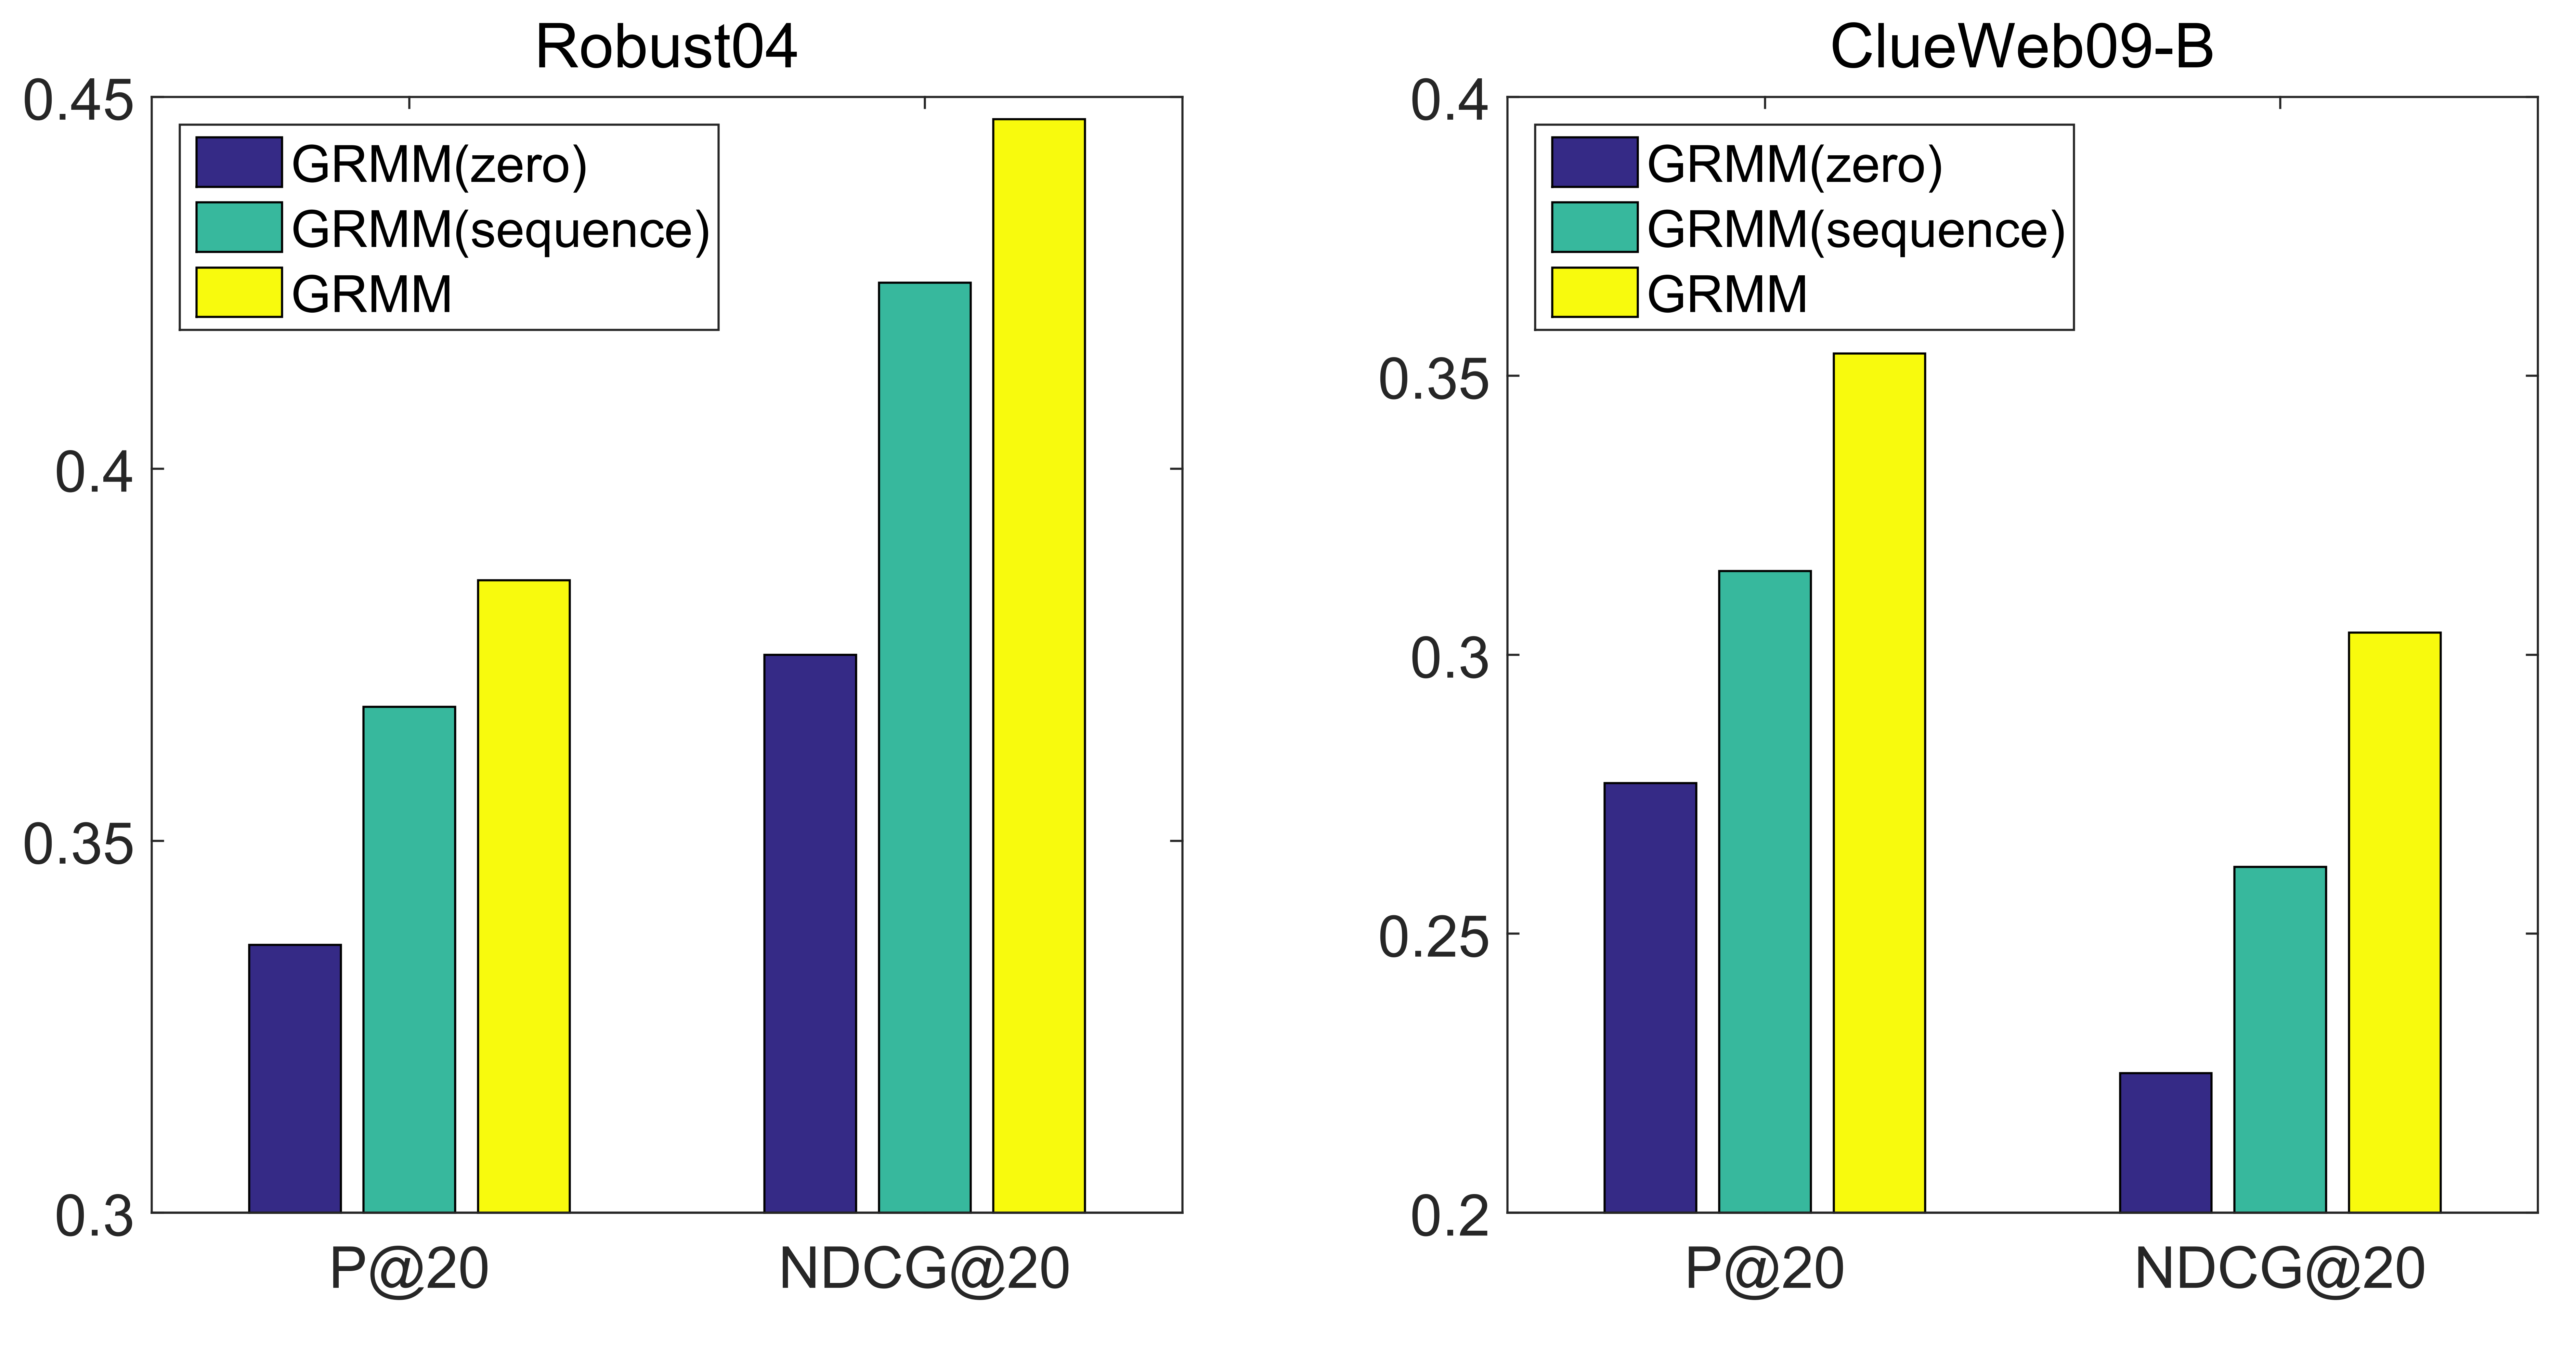
\includegraphics[width=.47\textwidth]{./pics/graph_ablation.png}
	\caption{Ablation study on graph structure of GRMM.}
	\label{fig:3} 
\end{figure}

Figure \ref{fig:3} illustrates the comparison between the original GRMM and the alternatives. We can see that:
\begin{itemize}
    \item GRMM (zero matrix) performs inferior to others in all cases. Since it merely depends on the junior term similarities, the model becomes approximate to term-based matching. Without contextualised refinement, some words and their synonyms can be misleading, which makes it even hard to discriminate the actual matching signals. 
    \item GRMM (word sequence) promotes GRMM (zero matrix) by fusing local neighbourhood information but still underperforms the original GRMM by a margin of 2-3 points. This observation resembles some results in Table \ref{tab:2}. It shows that such text format could advantage local context understanding but is insufficient in more comprehensive relationships. 
    \item  From an overall view of the comparison, the document-level word relationships along the graph structure is proved effective for ad-hoc retrieval. Moreover, a relatively greater gain on ClueWeb09-B indicates that longer texts can benefit more from the document-level respective field.
\end{itemize}

\subsection{Study of Neighbourhood Aggregation (RQ2 \& RQ3)}
\label{sec:neighbouraggre}
Figure \ref{fig:4} summarises the experimental performance w.r.t a different number of graph layers. The idea is to investigate the effect of high-order neighbourhood aggregations. For convenience, we notate GRMM-0 for the model with no graph layer, GRMM-1 for the model with a single graph layer, and so forth for the others. From the figure, we find that:

\begin{figure}[h]
	\centering
	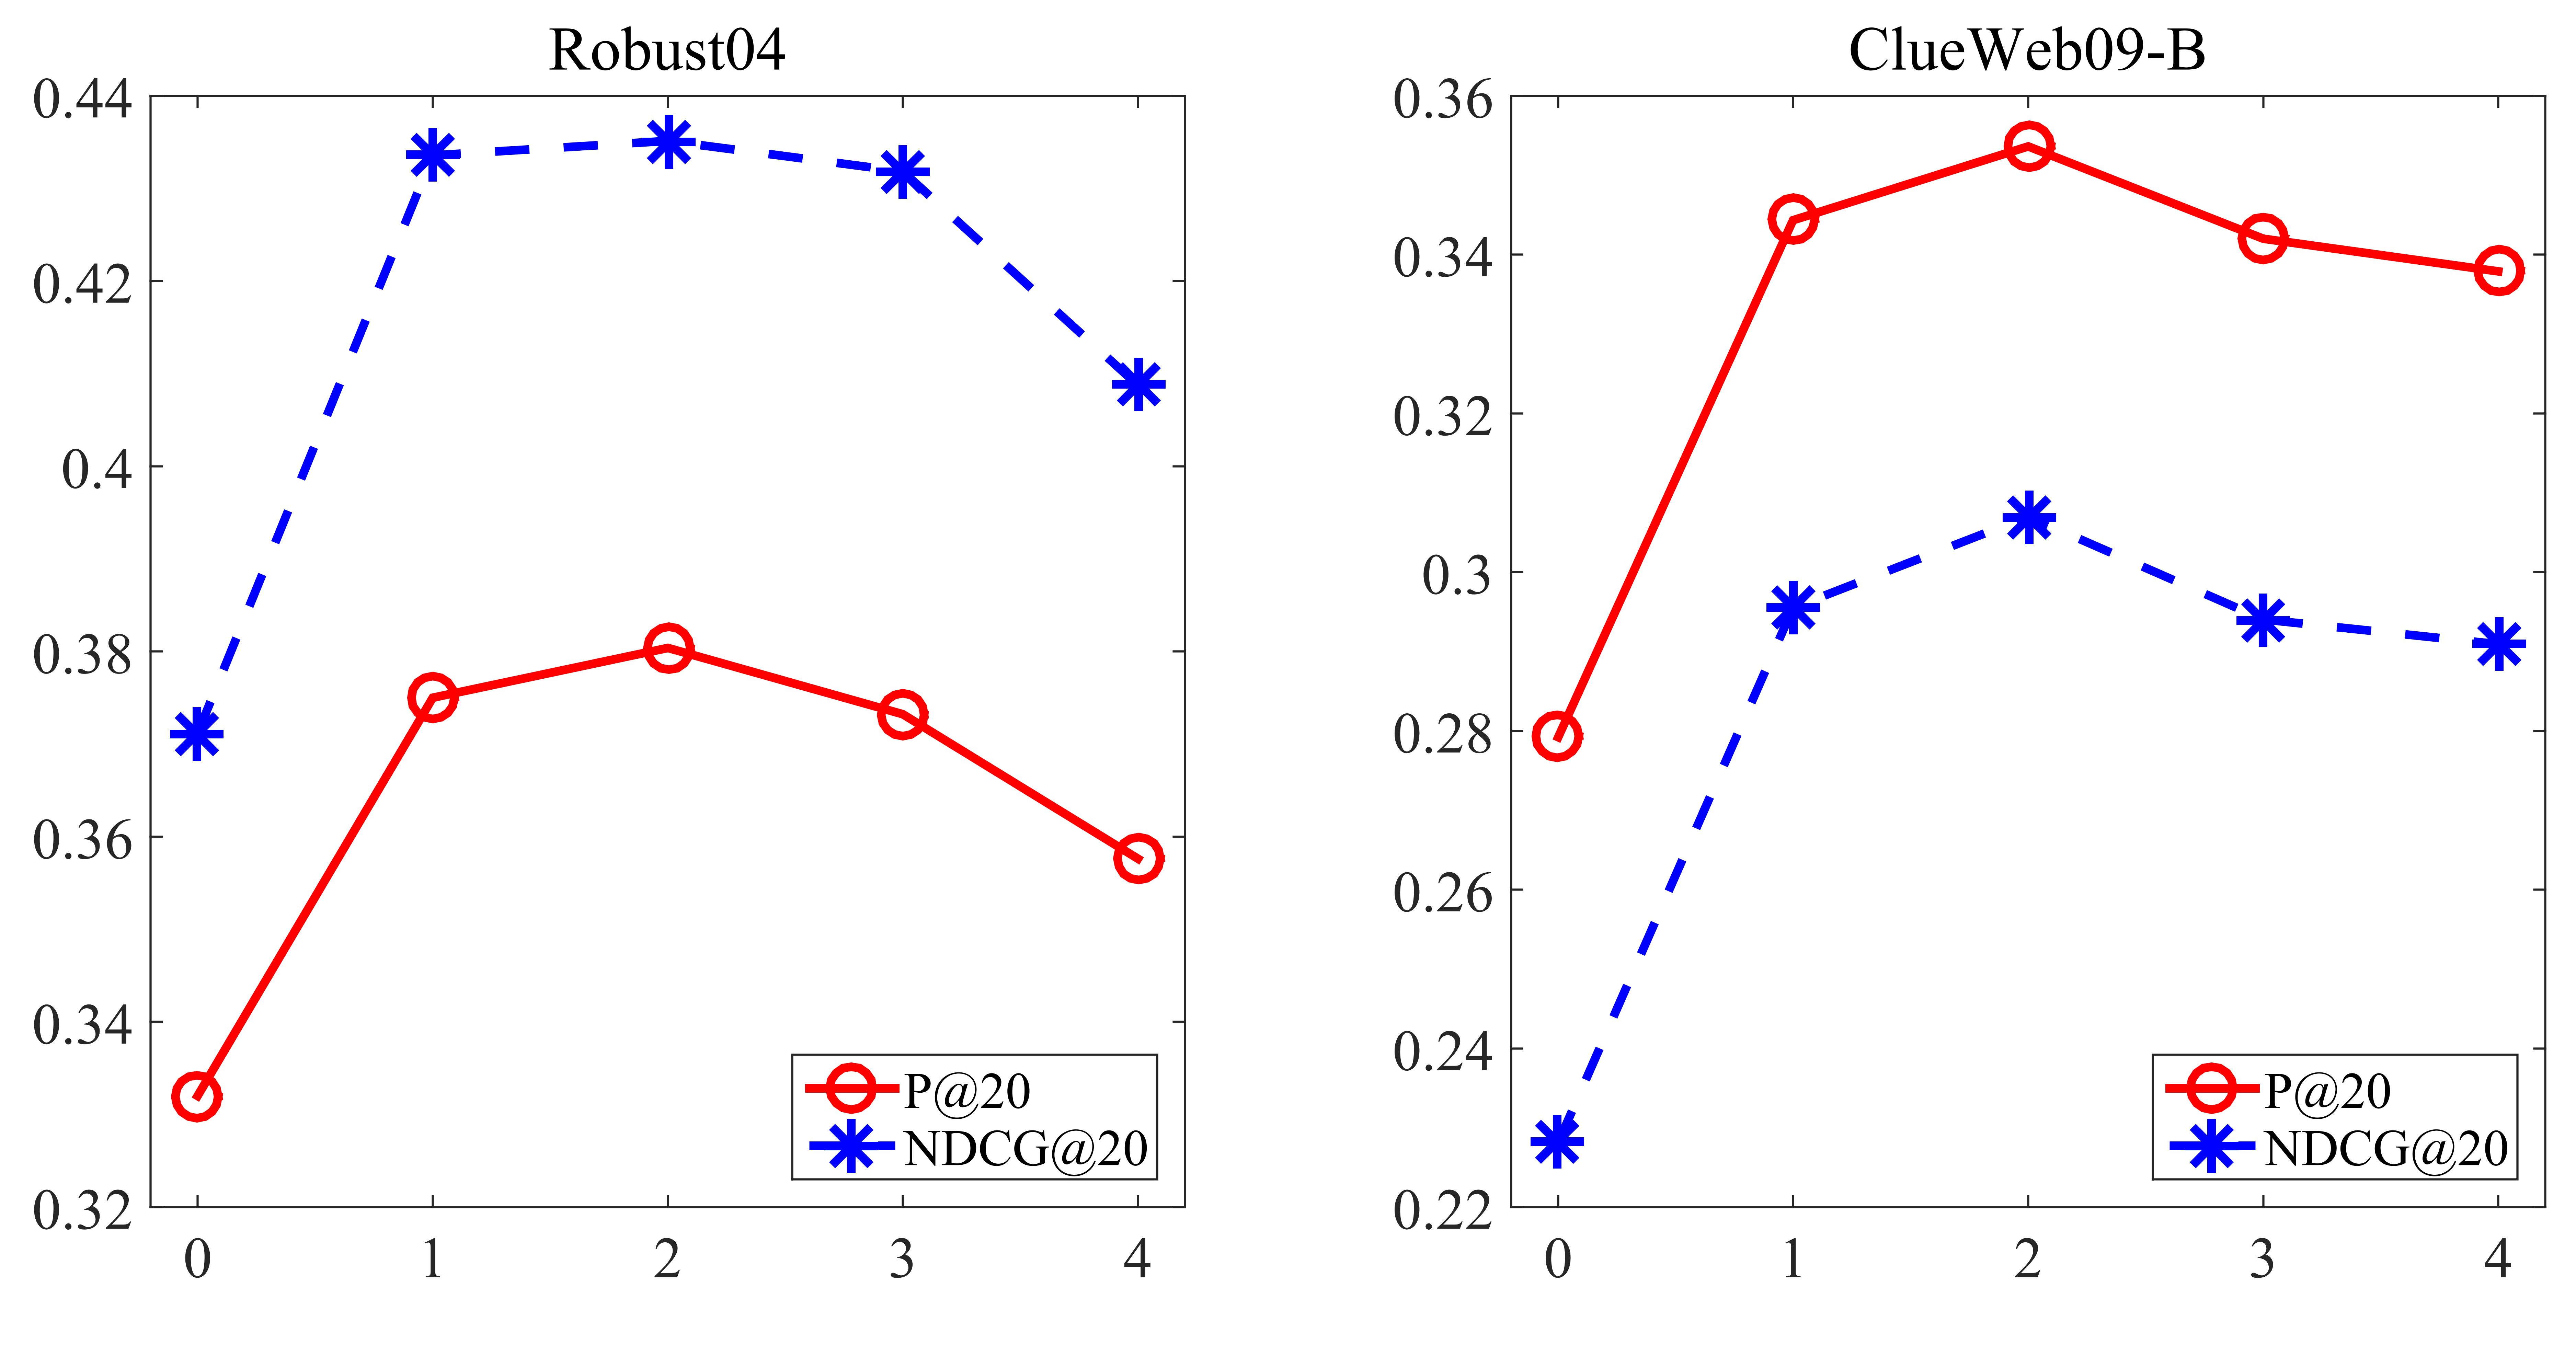
\includegraphics[width=.47\textwidth]{./pics/num_of_layers.png}
	\caption{Influence of different graph layer numbers.}
	\label{fig:4} 
\end{figure}

\begin{itemize}
	\item GRMM-1 dramatically boosts the performance against GRMM-0. This observation is consistent with Section \ref{sec:graphstructure} that propagating the information within the graph helps to understand both query-term interaction and document-level word relationships. The exact/similar query-document matching signals are likely to be strengthened or weakened according to intra-document word relationships. 
	\item GRMM-2 improves, not as much though, GRMM-1 by incorporating second-order neighbours. It suggests that the information from 2-hops away also contributes to the term relations. The nodes serving as a bridge can exchange the message from two ends in this way.
	\item However, when further stacking more layers, GRMM-3 and GRMM-4 suffer from slight performance degradation. The reason could be nodes receive more noises from high-order neighbours which burdens the training of parameters. Too much propagation may also lead to the issue of over-smooth \cite{kipf2017semi}. A two-layer propagation seems to be sufficient for capturing useful word relationships.
	\item Overall, there is a tremendous gap between using and not using the contextual information, and the model peaks at layer $t$ = 2 on both datasets. The tendency supports our hypothesis that it is essential to consider term-level interaction and document-level word relationships jointly for ad-hoc retrieval. 
\end{itemize}

\subsection{Study of Graph Readout (RQ3)}
\label{sec:featureelect}
\begin{figure}[h]
	\centering
	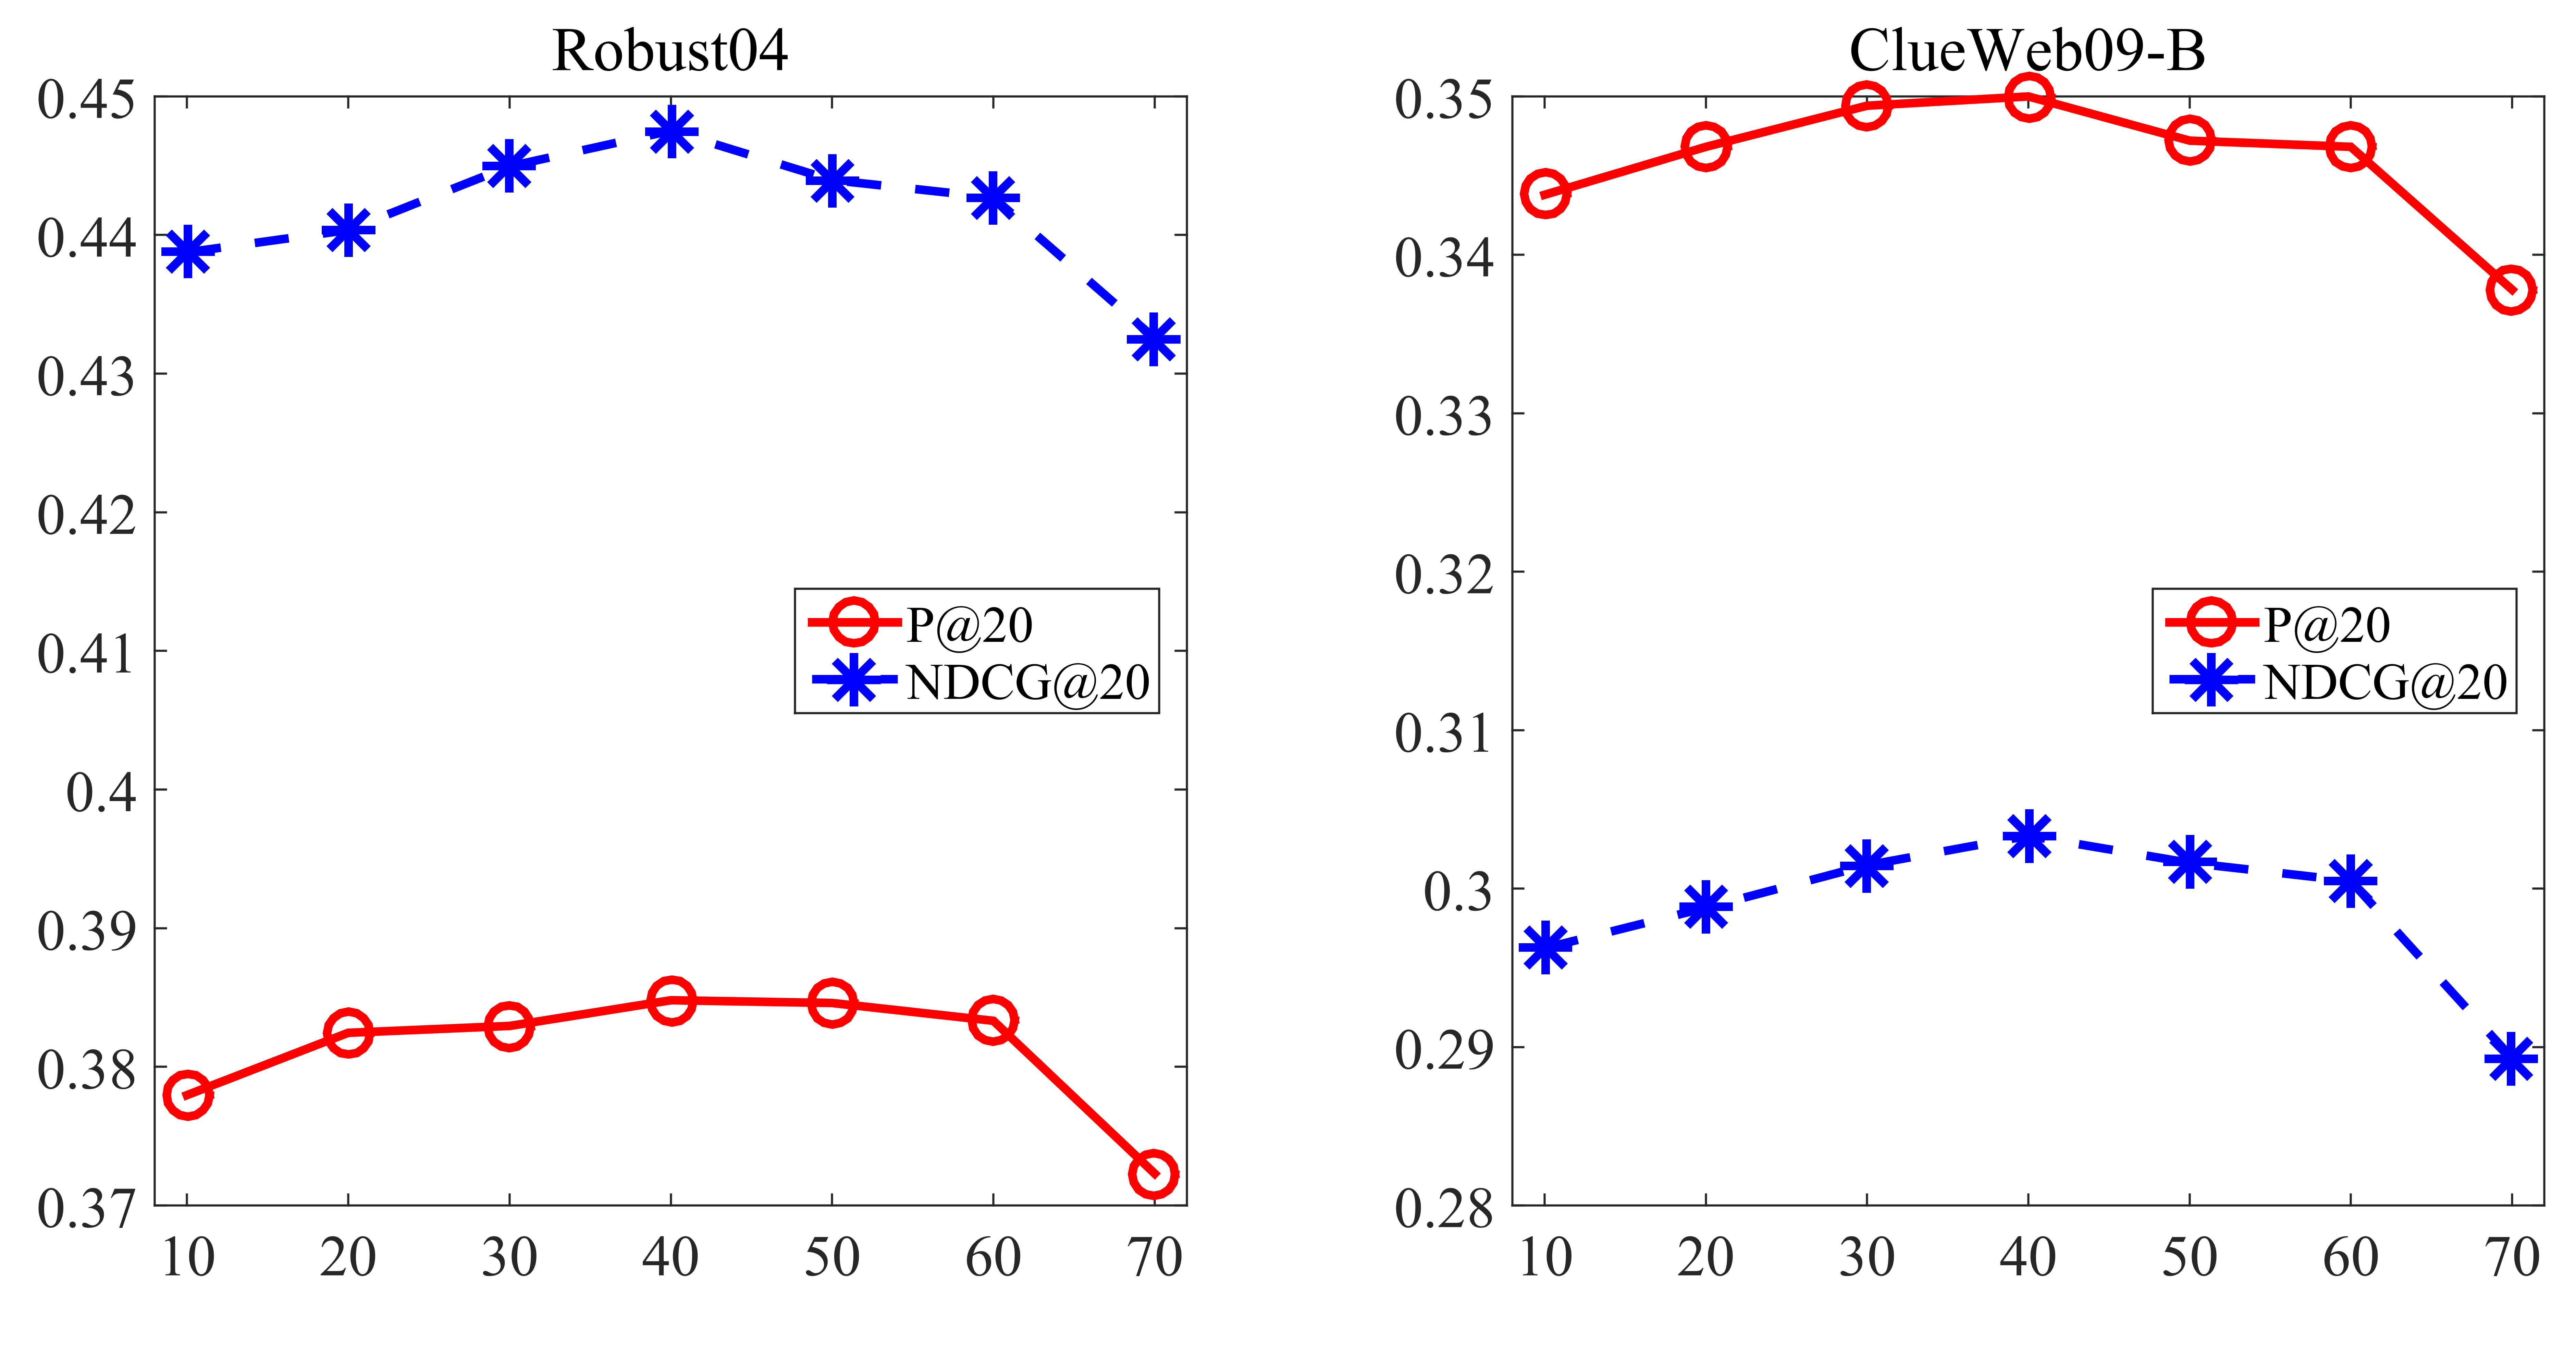
\includegraphics[width=.47\textwidth]{./pics/k.png}
	\caption{Influence of different $k$ values of $k$-max pooling.}
	\label{fig:5} 
\end{figure}

We also explored the effect of graph readout for each query term. Figure \ref{fig:5} summarises the experimental performance w.r.t different $k$ values of $k$-max-pooling. From the figure, we find that: 
\begin{itemize}
	\item The performance steadily grows from $k$ = 10 to $k$ = 40, which implies that a small feature dimension may limit the representation of terms. By enlarging the $k$ value, the relevant term with more matching signals can distinguish from the irrelevant one with less. 
	\item The trend, however, declines until $k$ = 70, which implies that a large feature dimension may bring negative influence. It can be explained that a large $k$ value may have a bias to the document length, where longer documents tend to have more matching signals. 
	\item Overall, there are no apparent sharp rises and falls in the figure, which tells that GRMM is not that sensitive to the selection of $k$ value. Notably, almost all performances (except $k$ = 70) exceed the baselines in Table \ref{tab:2}, suggesting that determinative matching signals are acquired during the graph-based interactions before feeding into the readout layer. 
\end{itemize}